\section{Umsetzung des realen Clusters}\label{sec:aufbauCluster}

\citeauthor{zhang2016} haben im Rahmen ihrer gesamten Forschungsarbeit die Open"=Source"=Plattform Hadoop"=Benchmark entwickelt und auf Github zur Verfügung gestellt.\footnote{\url{https://github.com/Spirals-Team/hadoop-benchmark}}
Sie wurde speziell zum Einsatz in der Forschung erstellt und kann jederzeit an die eigenen Bedürfnisse angepasst werden.
Zur Umsetzung des realen Clusters im Rahmen dieser Masterarbeit wurde daher eine speziell angepasste Version der Plattform eingesetzt.

\subsection{Plattform Hadoop"=Benchmark}\label{sec:hadoopBenchmark}

Die Plattform ist in mehrere Szenarien unterteilt, darunter ein Hadoop in der Version 2.7.1 ohne Änderungen und ein darauf basierendes Szenario mit der Selfbalancing"=Komponente.
Hadoop"=Benchmark basiert auf der Software \emph{Docker}\footnote{\url{https://www.docker.com/}} und dem dazugehörigen Tool \emph{Docker Machine}, um damit einfach und schnell ein Hadoop"=Cluster aufbauen zu können.
Mit \emph{Graphite}\footnote{\url{https://graphiteapp.org/}} ist zudem ein Monitoring"=Tool enthalten, mit dem die Performance des Clusters überwacht und analysiert werden kann.

\begin{figure}
    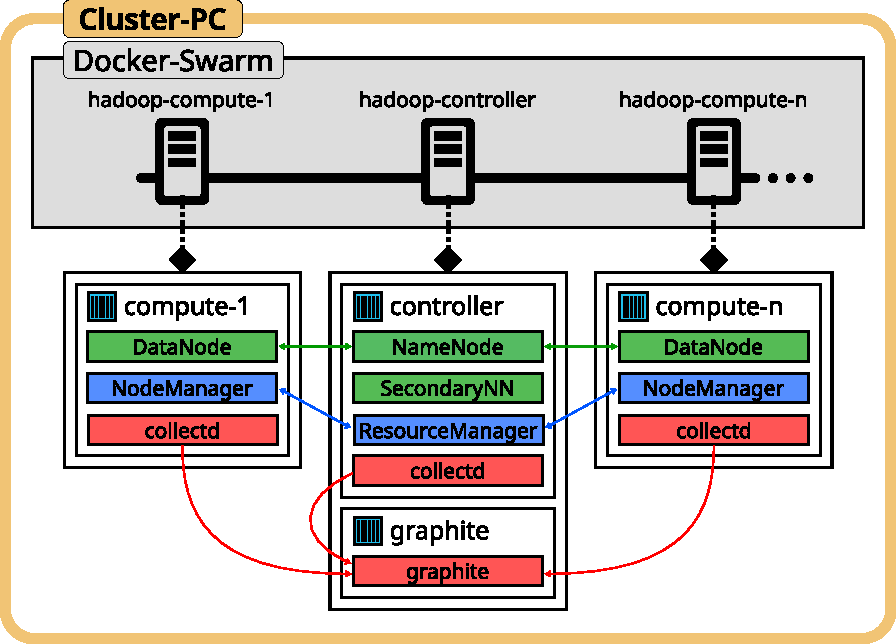
\includegraphics{./images/hadoopBenchmarkArch.pdf}
    \caption[High"=Level"=Architektur von Hadoop"=Benchmark]
    {High"=Level"=Architektur von Hadoop"=Benchmark.
        Grün: \ac{HDFS}, Blau: YARN, Rot: Graphite.
        \todo{In den nächsten Unterabschnitt verschieben}}
    \label{fig:hadoopBenchmarkArchitecture}
\end{figure}

\autoref{fig:hadoopBenchmarkArchitecture} zeigt die grundlegende Architektur der Plattform, die mithilfe eines Docker"=Swarms auf mehreren \emph{Docker Machines} (für den Einsatz von Docker eingerichtete virtuelle Maschinen) ein Cluster erstellt, auf denen dann in den Docker"=Containern das eigentliche Hadoop"=Cluster ausgeführt wird.
Jeder Hadoop"=Container enthält zudem das Tool \emph{collectd}\footnote{\url{https://collectd.org/}}, was das Monitoring des Containers auf Systemebene übernimmt und die Daten an den Graphite"=Container auf der Controller"=Machine übermittelt.
Es ist dabei möglich, eine beliebige Anzahl an Nodes zu nutzen.
Auch ist es möglich, den Docker Machines einen beliebig großen Arbeitsspeicher zur Verfügung zu stellen.

Die Plattform Hadoop"=Benchmark enthält zudem einige Benchmark"=Anwendungen:

\begin{itemize}
    \item Hadoop Mapreduce Examples
    \item Intel HiBench\footnote{\url{https://github.com/intel-hadoop/HiBench}}
    \item \ac{SWIM} \footnote{\url{https://github.com/SWIMProjectUCB/SWIM}}
\end{itemize}

Eine Besonderheit bildet der SWIM"=Benchmark, welcher sehr Ressourcenintensiv ist und daher auf einem \emph{Single Node Cluster}, also einem kompletten Hadoop"=Cluster auf nur einem Computer, sehr zeitintensiv sein kann.
Der Intel HiBench"=Benchmark besteht aus Kategorien wie \emph{Machine Learning} oder Graphen, welche wiederum aus einen oder mehreren \emph{Workloads} bestehen, welche entsprechende Anwendungen bzw. Algorithmen auf dem Hadoop"=Cluster ausführen.
Einige der Hibench"=Workloads basieren auf den Mapreduce Examples, welche wiederum voneinander unabhängige Beispielanwendungen für Hadoop darstellen.

\subsection{Anpassungen und Setup}\label{sec:clusterFallstudie}

Da mithilfe der Plattform Hadoop"=Benchmark die Erstellung eines Hadoop"=Clusters massiv vereinfacht wird, kommt die Plattform auch in dieser Masterarbeit zum Einsatz.
Da Docker und Hadoop vor allem für den Einsatz in einer Linux"=Umgebung entwickelt wurden, wird dazu ein eigener PC mit Ubuntu 16.04 LTS genutzt.
Da \sS das .NET"=Framework, und damit Windows, benötigt, wird dafür ebenfalls ein eigener PC verwendet.
Im konkreten Versuchsaufbau wird für Windows eine VM genutzt, welche auf einem anderen PC als das Cluster ausgeführt wird.
Beide zum Einsatz kommenden PCs sind jeweils mit einem Intel Core i5"=4570 @ 3,2 GHz x 4, 16 GB Arbeitsspeicher sowie einer insgesamt 512 GB großen SSD ausgestattet, auf der Ubuntu 16.04 LTS installiert ist.
%Die genauen Spezifikationen der PCs und der Windows"=VM sind in \autoref{tab:pcSpecs} aufgelistet.
Die Windows"=VM und der Cluster"=PC werden mithilfe von SSH"=Verbindungen miteinander verbunden.

%\begin{table}
%    \begin{tabular}{|c|c|c|c|}
%    	\hline
%    	 \textbf{}   & \textbf{Cluster"=PC} &          \textbf{VM"=PC}          & \textbf{Windows"=VM}  \\ \hline\hline
%    	\textbf{CPU} & \multicolumn{2}{|c|}{Intel Core i5"=4570 @ 3,2 GHz x 4} &     4 CPU Cores      \\ \hline
%    	\textbf{RAM} &        16 GB        &              16 GB               &         8 GB         \\ \hline
%    	\textbf{SSD} &       512 GB        &              512 GB              &  $\leq$ 100 GB VHD   \\ \hline
%    	\textbf{OS}  &  Ubuntu 16.04 LTS   &         Ubuntu 16.04 LTS         & Windows 10 1709 Edu. \\ \hline
%    \end{tabular}
%    \caption{Spezifikationen der verwendeten PCs und Windows"=VM}
%    \label{tab:pcSpecs}
%\end{table}

Auf dem Cluster"=PC nutzt Docker"=Machine zur Erstellung, Verwaltung und Ausführung der VMs die Treiber von VirtualBox 5.2\footnote{\url{https://www.virtualbox.org/}}, zum Abrufen der Daten der REST"=API über die SSH"=Verbindung wird \emph{curl}\footnote{\url{https://curl.haxx.se/}} genutzt.
Für das Cluster werden 4 Nodes, der Controller sowie eine Consul"=VM zur internen Verwaltung der Netzwerkverbindungen zwischen den VMs und Docker"=Containern erstellt.
Der Controller erhält 4 GB RAM, jeder der vier Nodes jeweils 2 GB, für den Consul sind 512 MB ausreichend.
Für die Windows"=VM wird ebenfalls VirtualBox 5.2 eingesetzt.

%TODO: Link zum angepassten Hadoop-Benchmark?
In keinem Szenario der Plattform Hadoop"=Benchmark wird standardmäßig der \ac{TLS} von Hadoop gestartet.
Daher wurde für diese Fallstudie basierend auf dem Selfbalancing"=Szenario ein neues Szenario erstellt, bei dem der \ac{TLS} gestartet wird.
Dadurch ist einerseits die Selfbalancing"=Komponente von \citeauthor{zhang2016} aktiv und andererseits besteht die Möglichkeit, für das Monitoring zusätzlich den \ac{TLS} zu nutzen.

Um die in dieser Fallstudie benötigten Befehle einfach ausführen zu können, wurden zwei eigene Scripte erstellt, welche, sofern möglich, auf den bestehenden Scripten der Plattform aufbauen.
Das Setup"=Script dient für folgende clusterbezogene Zwecke:

\begin{itemize}
    \item Starten, Beenden und Löschen des kompletten Clusters bzw. Hadoops
    \item Starten und Beenden des Docker"=Containers eines Hadoop"=Nodes
    \item Hinzufügen und Entfernen der Netzwerkverbindung des Docker"=Containers eines Hadoop"=Nodes
    \item Ausführen von eigenen Befehlen auf dem Docker"=Container des Controllers
\end{itemize}

Das zweite erstellte Script dient ausschließlich zum Starten der Benchmarks.

Für die Befehle, die das gesamte Cluster betreffen, wird vom Setup"=Script meist auf das in Hadoop"=Benchmark enthaltene Start"=Script zugegriffen.
Die Befehle, welche die Docker"=Container der Nodes betreffen, sowie das Ausführen von Befehlen im Controller"=Container, werden vom Setup"=Script direkt ausgeführt.
Für das Starten der Benchmarks werden dagegen die in Hadoop"=Benchmark enthaltenen Ausführungs"=Scripte der Benchmarks gestartet.
